% !TEX program = xelatex
\documentclass[tikz, crop, border = {2pt 2pt 2pt 2pt}]{standalone}

\usepackage{concmath-otf}
\usetikzlibrary{calc, angles, quotes, patterns, decorations.pathreplacing, decorations.pathmorphing, calligraphy, arrows.meta}
\usetikzlibrary{math}
\usepackage{physics2}
\usepackage{derivative}
\usephysicsmodule{ab, ab.braket, ab.legacy, nabla.legacy, op.legacy}

\begin{document}
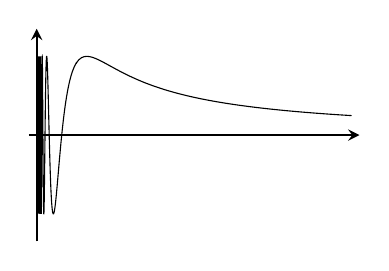
\begin{tikzpicture}
  \tikzstyle{axis} = [thick, -stealth]
  \draw[axis] (-0.1, 0) -- (4.1, 0);
  \draw[axis] (0, -1.35) -- (0, 1.35);
  \draw[domain = 0.5:4, samples=100, smooth] plot (\x, {sin((1/\x) r)});
  \draw[domain = 0.02:0.51, samples=2000, smooth] plot (\x, {sin((1/\x) r)});
\end{tikzpicture}
\end{document}
